\documentclass[12pt, a4paper, twoside]{article} %landscape,

\usepackage{enumitem}
\usepackage[utf8x]{inputenc}
\usepackage[T1]{fontenc}
\usepackage[frenchb]{babel}
\usepackage{tabularx}
\newcolumntype{Y}{>{\centering\arraybackslash}X}
\usepackage{multirow}
\usepackage{gensymb} % Symbole générale 
\usepackage{lmodern}
\usepackage{lastpage} % dernière page 
\usepackage{graphicx}% pour les graphiques
\usepackage[top=2.5cm, bottom=2.5cm, left=2.5cm, right=2.5cm]{geometry}
\usepackage{framed} % crée 3 environnement : shaded, framed, left­bar
\usepackage{amsmath, amssymb, mathrsfs} % pour les maths
\usepackage[H]{float}
%\usepackage{fancybox} % permet de faire des boite et d'encadrer 
%\usepackage{float} 
%\usepackage{subcaption}
% définition des en tête pied de pages 
\usepackage{fancyhdr} % entête et pied de page
\pagestyle{fancy}
\fancyhead[L]{
\includegraphics[scale=0.3]{insa.pdf}}
\fancyhead[C]{TP Perte de charge}
%Étude d'une flamme de prémélange 
\fancyhead[R]{\date{Le 27 mars 2020 }}
%\scriptsize{\leftmark}
%\leftmark
\fancyfoot[R]{}
\fancyfoot[C]{Page \thepage \, sur \pageref{LastPage}}
\fancyfoot[L]{}
%\renewcommand{\headrulewidth}{2pt} % changer la largeur de la ligne en desssous 
\renewcommand{\thesection}{\Roman{section}} % change numérotation section
\usepackage{appendix} % Annexes 

\usepackage[table]{xcolor}% charge les couleurs dans les tableaux
\usepackage{lscape}
\date{Le 27 mars 2020} % date du compte rendu 
%\usepackage{appendix} % Annexes
\title{Note de synthèse TP hydraulique : \'Etude de pompes centrifuges } % titre du document 
\author{Benoit \textsc{Saunier} \& Christophe \textsc{Monnier} \& Thomas \textsc{Boutron} \& Damien \textsc{Bouvier} \\  Groupe 3, binôme 9 et 10 ; \thedate} % nom des auteurs 

\renewcommand{\r}{\right)}
\renewcommand{\l}{\left(}

\begin{document}
\renewcommand{\contentsname}{Sommaire}
\input{Cover_Page.tex}
\newpage 
\tableofcontents
\newpage

%\maketitle % permet d'afficher le titre 
\section*{Nomenclature}

\begin{table}[H]
    \centering
     \caption{Table des nomenclatures}
    \begin{tabular}{|c|c|c|c|}
    \multicolumn{4}{c}{ }\\
       \hline
        \textbf{Nom} & \textbf{symbole} & \textbf{unité} &\textbf{Valeur} \\
        \hline
        Diamètre & D & \multirow{7}{*}{$m$} &\multirow{12}{*}{/}\\
        \cline{1-2}
        Longueur de tube & L &  & \\
         \cline{1-2}
         Altitude & z &  & \\
         \cline{1-2}
         Hauteur piézométrique & $H_{p}$ &  & \\
         \cline{1-2}
         Hauteur manométrique & $H_{m}$ &  & \\
         \cline{1-2}
        Rayon de courbure de coude & r &  &\\
         \cline{1-2}
         Charge & C &  &\\
         \cline{1-2}
        Perte de charge & J &  & \\
        \cline{1-3}
        Angle d'un coude & $\beta$ & $\degree$ & \\
        \cline{1-3}
        Vitesse du fluide & U& $m\cdot s^{-1}$ & \\
        \cline{1-3}
        Débit du fluide & $Q_v$ & $m^{3}\cdot s^{-1}$ & \\
       \cline{1-3}
       Surface de passage de la canalisation & $S_i$ & $m^{2}$ & \\
       \cline{1-3}
        Pression du fluide & $P_i$ & $kg\cdot m^{-1}\cdot s^{-2}$ & \\
       \cline{1-3}
        Nombre de Reynolds & Re & \multirow{3}{*}{$1$}& \\
       \cline{1-2}
        Coefficient pertes de charge régulières & $\lambda$  &  & \\
        \cline{1-2}
        Coefficient pertes de charge singulières & K&  &\\
        \cline{1-3}
        Masse volumique & $\rho$&  $kg\cdot m^{-3}$&\\
        \hline
        Accélération de la pesanteur & g & $m\cdot s^{-2}$ & 9,81\\
        \hline
        Viscosité cinématique de l'eau & $\nu$ & $m^2 \cdot s^{-1}$& $10^{-6}$\\
        \hline
    \end{tabular}
    \label{tab:nomenclature}
\end{table}


\clearpage
\section{Introduction } 

L'objectif de la manipulation présentée ici est de comparer les prédictions théoriques des pertes de charges dans un circuit d'eau à des mesures expérimentales. Dès qu'un fluide est transporté à travers des conduites, sa charge (en quelque sorte son énergie) diminue au fur et à mesure de son cheminement. Cette diminution est due aux dissipations d'énergie liées aux forces de viscosité sur l'interface paroi-fluide. 
En hydraulique, deux types de pertes de charges peuvent être distinguées : Les pertes de charge régulières et les pertes de charge singulières. \\
Les pertes de charge régulières représentent la diminution de la charge lors de la progression du fluide dans une conduite droite (sans "singularité"). La mécanique des fluides nous dit que la perte de pression du fluide varie linéairement avec la longueur parcourue. 
\\ Les pertes de charge singulières sont dues à des singularités géométriques. En effet, lorsque le fluide passe par un coude ou un élargissement, les pertes de pressions sont assez importantes et la régime d'écoulement du fluide est perturbé par des décollements et des turbulences.

La connaissance et la prédiction des pertes de charge dans une conduite sont essentielles pour pouvoir prévoir quelles pompes ou turbines utiliser, ou encore savoir si l'on risque d'avoir de la cavitation (phénomène de formation de poches de gaz, très néfaste pour le fonctionnement d'un système hydraulique) dans la canalisation ou la turbomachine.


\section{Banc d'essai et protocole }

Le banc d'essai représenté sur la figure~\ref{fig:instal} est constitué de deux circuits qui seront étudiés séparément. 
\begin{figure}
    \centering
    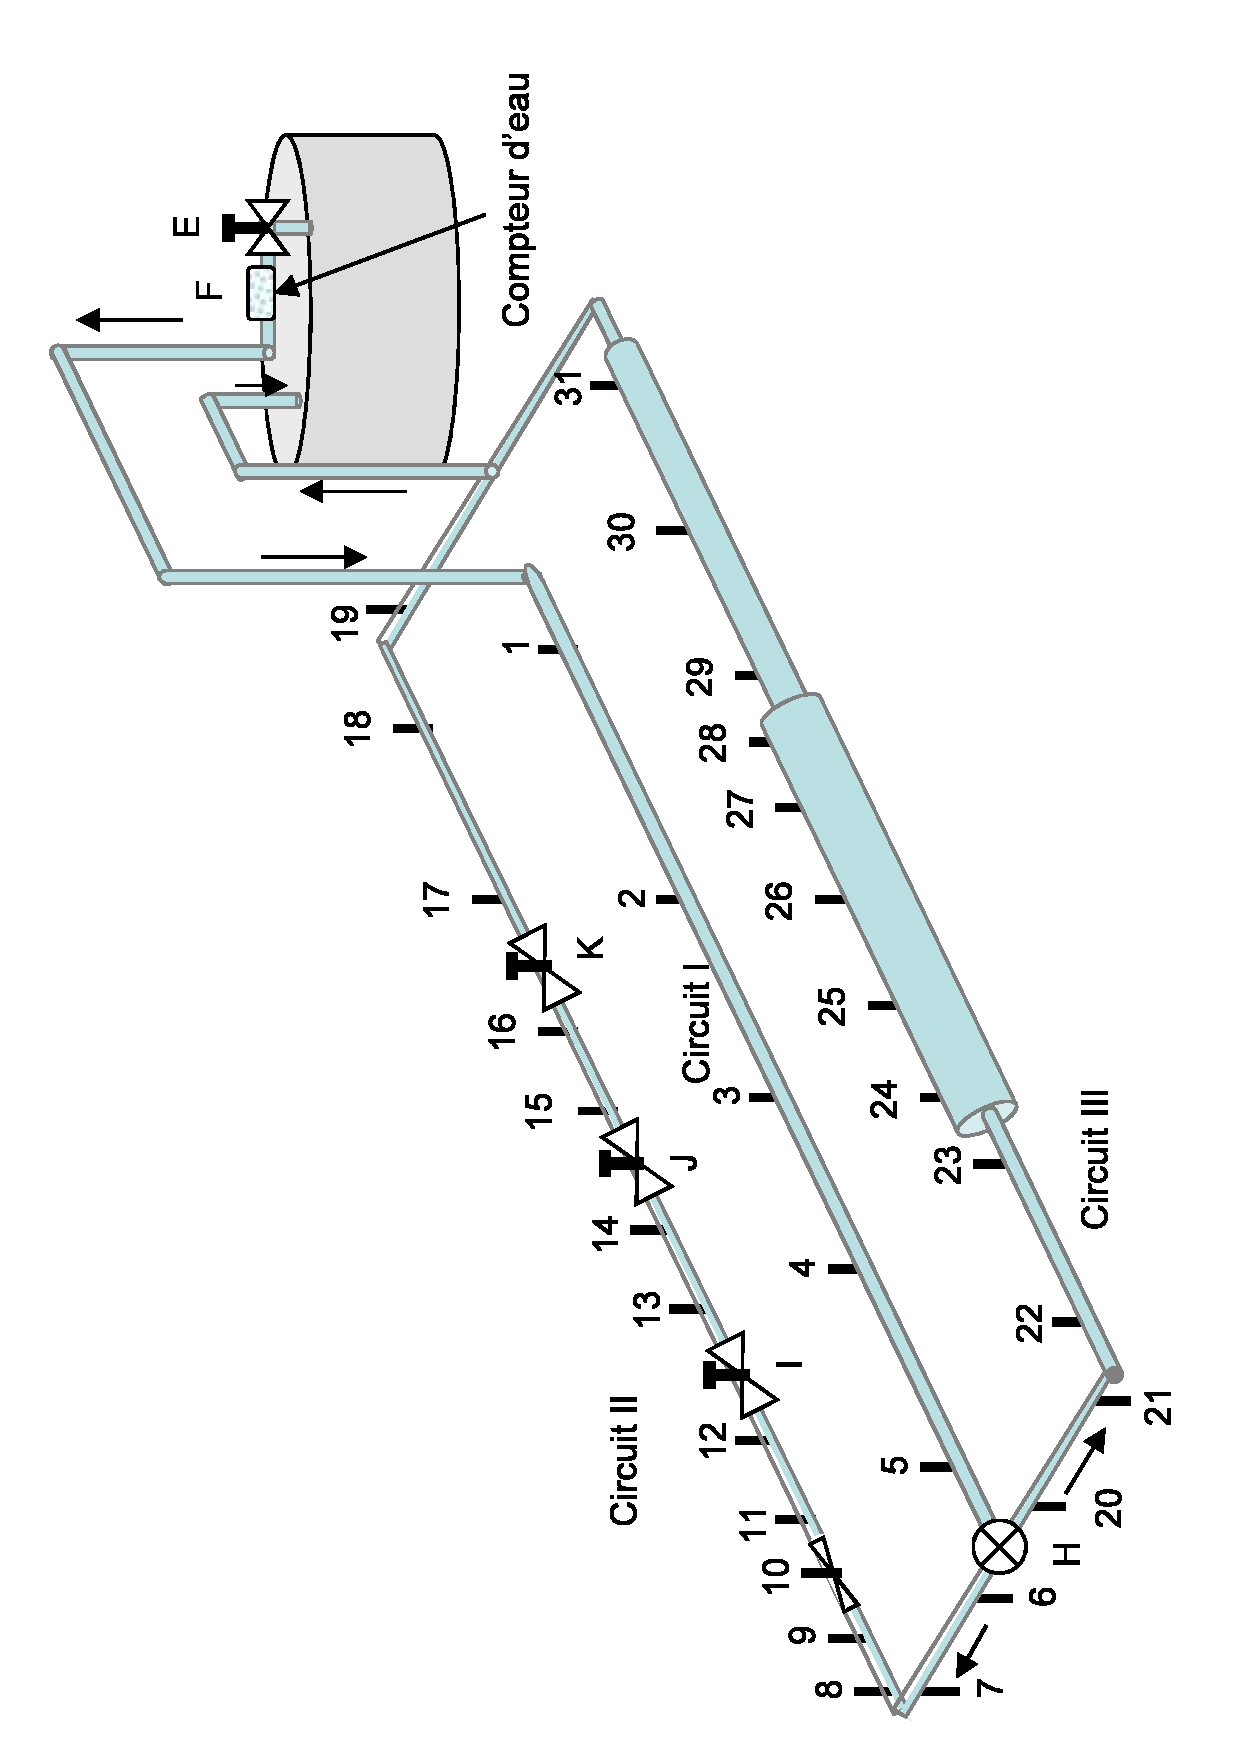
\includegraphics[angle=-90, width = \linewidth]{instal.pdf}
    \caption{Schéma de l'installation étudié}
    \label{fig:instal}
\end{figure}

Sur la figure~\ref{fig:instal} nous voyons qu'un grand réservoir d'eau, dans lequel est installée une pompe  qui est le fournisseur de débit de notre installation. On remarquera que celle-ci fonctionne en circuit fermé (l'eau revient dans le réservoir) afin d'économiser l'eau. L'eau pompée du réservoir passe d'abord par le circuit I, droit et régulier. Au bout de celui-ci se trouve une vanne 3 voies notée H, qui oriente l'eau soit pour aller dans le circuit II soit dans le circuit III.
\\Le circuit II, outre le fait de comporter des coudes, comporte aussi différentes vannes et un dispositif de mesure de débit Venturi.
\\Le circuit III comporte un élargissement puis un rétrécissement de section.
\\Sur tout le long des circuits I, II et III de nombreux points de mesure de pression sont présents. Ils permettront notamment de suivre l'évolution de la charge.

\subsection*{Protocole expérimental } 
Les objectifs principaux du TP sont : 
\begin{itemize}
    \item \'Etudier les différents types de pertes de charges, les différentes singularités et leurs impacts;
    \item Comparer le débit mesuré grâce à un venturi et un compteur volumétrique ;
    \item Déduire expérimentalement le coefficient de perte de charge K d'une vanne 3 voies; 
    \item Comparer les résultats expérimentaux et théoriques.
\end{itemize}

L'équation de Bernoulli généralisée (équation~(\ref{eq:bernoulli})) permet de déterminer la charge C en un point donné du réseau hydraulique. 
Afin d'étudier le comportement du fluide sur chaque partie du réseau, un  bilan entre deux point sera fait (équation (\ref{eq:bilan_charge})) : 

\begin{equation}
    C = \frac{P}{\rho \, g} + \frac{U^2}{2 \, g} + z
    \label{eq:bernoulli}
\end{equation}

\begin{equation}
   C_j = C_i + \sum J_{ij} + H_m
    \label{eq:bilan_charge}
\end{equation}
\clearpage
\section{Résultats et exploitation :}

\subsection{Pertes de charges régulières : }
Pour déterminer la perte de charge régulière J liée à un longueur L d'une canalisation de diamètre D il faut utiliser l'équation~(\ref{eq:Jreg}) :
\begin{equation}
    J=\lambda\frac{L}{D}\frac{U^{2}}{2g}
    \label{eq:Jreg}
\end{equation}

Où le coefficient $\lambda$ dépend généralement du régime d'écoulement et de la rugosité de la paroi (Les parois des conduites sont ici considérées comme lisses). Ici, compte tenu du fait que le nombre de Reynolds $Re$ (calculé à l'aide de la formule ~(\ref{eq:Re})) est compris entre 2000 et 50 000, la formule~(\ref{eq:lambda}) est utilisée pour calculer $\lambda$. La vitesse $U$, utilisée pour calculer le Reynolds et les pertes de charges est calculée grâce au débit trouvé grâce au compteur volumétrique dans le tableau~\ref{tab:mesure_débit}. 

\begin{equation}
    Re=\frac{D\, U^{2}}{\nu}
    \label{eq:Re}
\end{equation}

\begin{equation}
    \lambda=\frac{0,316}{Re^{0,25}}
    \label{eq:lambda}
\end{equation}
 
 Toutes les pertes de charges et leurs composante sont calculées dans les tableau~\ref{tab:Valeurs_theo_II} et ~\ref{tab:Valeurs_theo_III} (voir annexe~\ref{Annexe:Données et valeurs calculer, circuit I,II} et \ref{Annexe:Données et valeurs calculer, circuit I,III}).  


\subsection{Pertes de charges singulières : }
Les pertes de charge singulières peuvent être déterminées grâce à la connaissance du coefficient K, qui est d'autant plus grand que la singularité géométrique est "brutale" et donc entraîne des turbulences et décollements important dans le fluide. L'équation (\ref{eq:Jsing}) est utilisée pour les calculer.

\begin{equation}
   J=K\frac{U^{2}}{2g}
    \label{eq:Jsing}
\end{equation}
 Toutes les pertes de charges et leurs composante sont calculées dans les tableau~\ref{tab:Valeurs_theo_II} et ~\ref{tab:Valeurs_theo_III} (voir annexe~\ref{Annexe:Données et valeurs calculer, circuit I,II} et \ref{Annexe:Données et valeurs calculer, circuit I,III}).  
 
La détermination de K est parfois compliquée, soit il faut se reporter à la littérature (quand c'est possible), soit il faut estimer la valeur via des mesures, c'est ce qui sera fait dans la prochaine sous section pour la vanne trois voies du circuit.



\subsection{Détermination K expérimental }

%Il est plus difficile de déterminer le coefficient $K_{H}$ de la vanne H car il ne faut pas se reporter à la perte de charge annoncée par les manomètres. Cette perte de charge est négative (ce qui est physiquement impossible, une telle perte de charge correspondrait à un apport d'énergie au fluide juste du fait son mouvement), et cela est dû au fait que la prise de pression est trop proche de la vanne. L'écoulement est n'est pas établi et les mesures sont donc faussées par les turbulences. il faut prendre les mesures loin de cette singularité pour être en régime établi. \\
%Les pertes de charges aux points 7 et 21 sont donc négatives et ces points ne sont donc pas à prendre en compte lors du tracé.
Il est plus difficile de déterminer le coefficient $K_{H}$ de la vanne H car il ne faut pas se reporter aux pertes de charges associés à la hauteur piézométrique annoncée par les manomètres. Cette perte de charge est négative (ce qui est physiquement impossible, une telle perte de charge correspondrait à un apport d'énergie au fluide juste du fait son mouvement), et cela est dû au fait que la prise de pression est trop proche de la vanne. L'écoulement est n'est pas établi et les mesures sont donc faussées par les turbulences. il faut prendre les mesures loin de cette singularité pour être en régime établi. \\
La hauteur piézométrique relevée entre les points 7 et 21 étant fausse, les pertes de charges calculées à partir des différences de hauteurs sont fausses. Ces points ne sont donc pas à prendre en compte lors du tracé.

Sachant que les pertes de charges $J_{reg,6,7}$ s'obtiennent via la formule (\ref{eq:Jreg}) et que $C_{5}$ et $C_{7}$ sont connus, en combinant les équations (\ref{eq:bilan_charge}) et (\ref{eq:Jsing}) il vient l'équation (\ref{eq:KH2}):
\begin{equation}
   K_{H}=(C_{5}-C_{7}-J_{reg,6,7})\frac{2g}{U^{2}}
    \label{eq:KH2}
\end{equation}
La valeur du coefficient K est dans le tableau~\ref{tab:Valeurs_theo_II}. 

Il faut remarquer que dans notre cas, dans l'équation (\ref{eq:bilan_charge}), $H_{m}$ est nul car il n'y a pas de machine.
\\
\subsubsection*{Remarque}
Les valeurs aberrantes de pertes de charge aux points 25 et 26 sont dus à un élargissement brusque. Les lignes de courant se décollent, il faut attendre assez longtemps pour que l'écoulement se rétablisse. Il ne faut donc pas prendre en compte ces pertes de charges négatives.

\subsection{Mesure du débit à l'aide du Venturi et d'un débimètre}

Le Venturi est un organe déprimogène constitué d'une réduction de diamètre de la canalisation, augmentant la vitesse du fluide et diminuant sa pression puis d'une augmentation de diamètre produisant l'effet inverse. Connaissant la différence de pression entre les points 10 et 9 du circuit correspondant à la dépression induite par le Venturi et les sections du Venturi, il est possible de remonter au débit de l'écoulement en combinant l'équation de Bernoulli (équation (\ref{eq:bernoulli})) et l'équation de conservation du débit (\ref{eq:debit}). L'application de Bernoulli se fait entre les points 9 et 10, respectivement avant et après l'organe déprimogène du tube de Venturi. On obtient finalement l'expression \ref{eq:venturi}.

\begin{equation}
   Q_{v} = U_9S_9 = U_{10}S_{10}
    \label{eq:debit}
\end{equation}

\begin{equation}
   Q_{v} = S_9\sqrt{\frac{2}{\rho}\frac{P_9 - P_{10}}{(\frac{S_9}{S_{10}})^2-1}}
    \label{eq:venturi}
\end{equation}

Afin de mesurer le débit circulant dans la canalisation, un compteur volumétrique et un chronomètre ont été utilisés afin de mesurer le débit. Les résultats des mesures sont compilés dans le tableau~\ref{tab:mesure_débit} dans l'annexe~\ref{Annexe:Données et valeurs calculer}. 
Ainsi, un débit de $1,53.10^{-3} m^3$ est trouvé grâce au compteur volumétrique et un débit de $1,62.10^{-3} m^3$ avec le Venturi.
%\begin{table}[H]
%    \centering
%    \caption{Résultats des mesures de débit}
%    \begin{tabular}{|c|c|}
%    \multicolumn{2}{c}{ } \\
%      \hline
%      Organe de mesure & débit $Q_v$  \\
%      \hline
%      Débitmètre & $1,53\times 10^{-3}$ \\
%      \hline
%      Venturi & $1,61\times 10^{-3}$ \\
%      \hline
%   \end{tabular}
%   \label{tab:debit}
%\end{table}
%Les résultats de mesures qui sont compilés dans le tableau~\ref{tab:mesure_débit} dans l'annexe~\ref{Annexe:Données et valeurs calculer} nous montre que 
L'ordre de grandeur du débit reste le même quel que soit l'organe de mesure utilisé. La légère variation pourrait s'expliquer par l'absence de prise en compte des pertes de charge du Venturi dans les calculs.


\subsection{Analyse des lignes de charges, piézométrqiues et altitudes } % j'ai enlevé le "vide en trop" et j'ai rajouter "Analyse des". 

\begin{figure}[H]
    \centering
    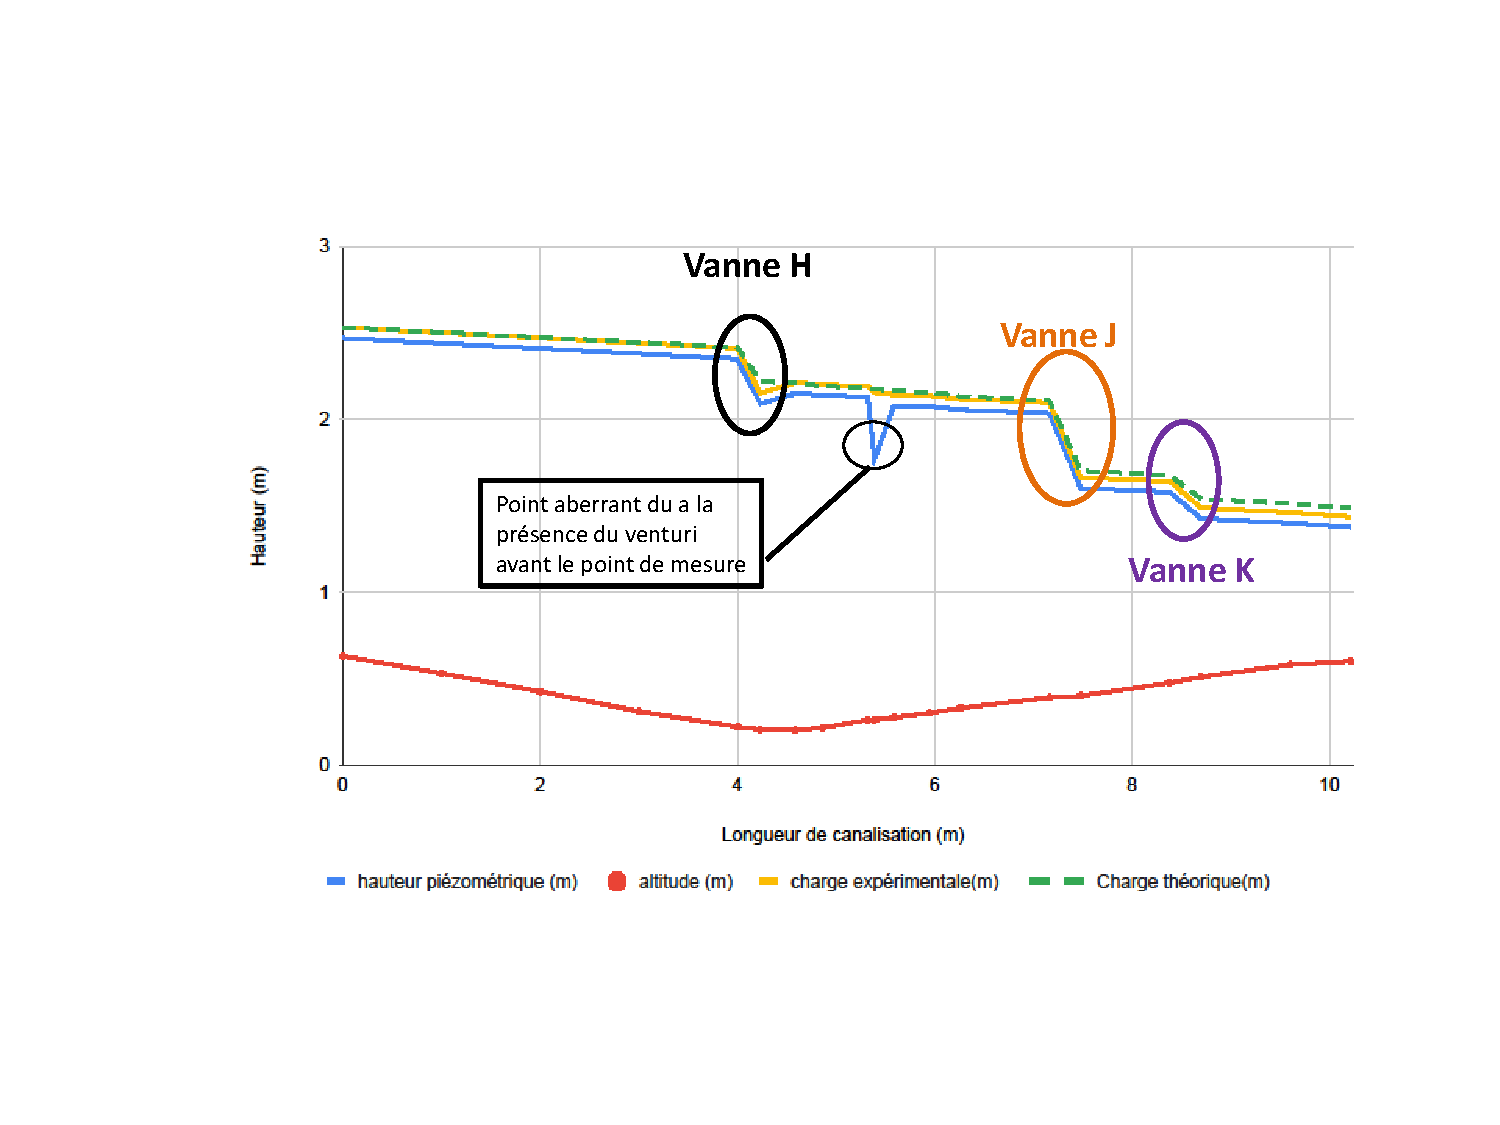
\includegraphics[ width = \linewidth]{Graph_II_2.pdf}
    \caption{\'Evolution de la hauteur en fonction de la longueur de tuyau du circuit I - II}
    \label{fig:graph_II}
\end{figure}

\paragraph{Exploitation figure~\ref{fig:graph_II}} 
Les courbes tracées sur la figure~\ref{fig:graph_II} représentent les différents termes de l'équation de Bernoulli (équation~\ref{eq:bernoulli}). La ligne d'altitude étant le terme "z", la ligne piézométrique prenant en compte les termes $\frac{P}{\rho g} + z $ et la ligne de charge C prenant en compte tout les termes de l'équation de  Bernoulli. \\
Lorsque les courbes bleu, jaune et verte sont linéaires cela indique qu'aucune singularité n'est présente. Il n'y a donc que les pertes de charges régulières qui induisent une diminution de hauteur. 

La ligne piézométrique décroît de manière linéaire avec l'altitude et les pertes de charge régulières. Les changement de pente sont dus aux pertes de charges singulières de l'installation.

Il est possible de remarquer que les courbes de charges expérimentales et théoriques sont confondues sur presque toute la longueur de la canalisation. Les points de décrochage se trouvent après les singularités créant une chute de charge et un point de mesure aberrant. La vanne I ne crée pas de perte de charges significativement visible sur le graphique \ref{fig:graph_II} étant donné que son coefficient de pertes de charge singulières est très faible.\\
Il est observable que la pente d'altitude est décroissante puis croissante ce qui indique que l'installation étudiée est en pente et que le point le plus bas se situe après la vanne H. Une fois passé le point  De plus, la ligne d'altitude est toujours inférieure aux autres lignes. Les risques de cavitations sont donc nuls dans cette installation.

%\includegraphics[trim = 3cm 17cm 1cm 1cm, clip]{dessin3_exam_juin_2010}
%coupe à gauche, en bas, à droite et en haut
\begin{figure}[H]
    \centering
     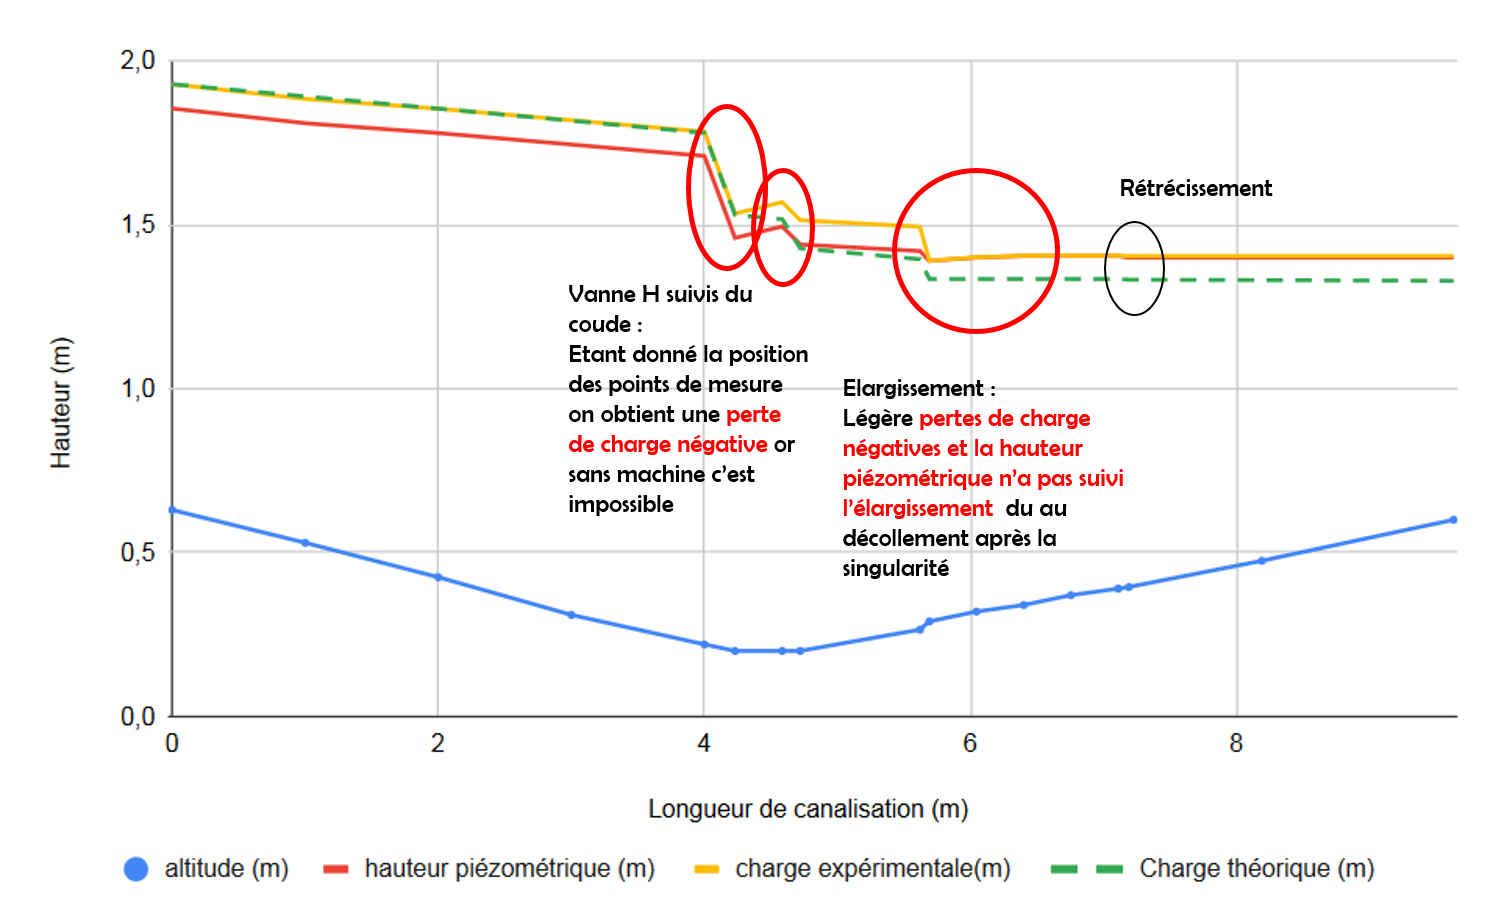
\includegraphics[width = \linewidth]{graph_I_III.png}
    \caption{\'Evolution de la hauteur en fonction de la longueur de tuyau du circuit I - III}
    \label{fig:graph_III}
\end{figure} 

\paragraph{Exploitation figure~\ref{fig:graph_III}}

Comme pour la figure \ref{fig:graph_II} les différents tracés représentes les différents termes de l'équation de Bernoulli. Les mêmes remarques que pour la figure \ref{fig:graph_II} sur l'origine des décrochements s'appliquent ici.La ligne de charge apparaît horizontale à partir de 5,5 m car le gain d'altitude compense les pertes de pression dans le calcul de la charge. %correction demandée par Sartre On va voir ce qu'elle dit 


\section{Conclusion}

L'expérience menée a permis de soulever plusieurs remarques importantes concernant l'étude des pertes de charges dans un circuit hydraulique. La plus importante est qu'il faut être critique par rapport aux tracés des lignes de charges expérimentales. En effet des points de mesure de pression sont mal placés (trop près de singularité géométriques comme des vannes) peuvent mener à des "gains de charges" dans le fluide, ce qui n'est pas le cas en réalité, puisque aucune machine n'est présente. Certaines singularités entraînent en effet des décollements des lignes d'écoulement et donc des dépressions, ce qui peut induire en erreur. \\
Il a aussi été vérifié que toutes les vannes n'ont pas le même impact sur les pertes de charges, certaines en entraînant de très importantes (la vanne à soupape J) alors que d'autres non (la vanne à passage direct I). D'ailleurs le coefficient de perte charge singulière de la vanne J a pu être déterminé grâce à des mesures.
\\Enfin, les tracés montrent que le modèle théorique des pertes de charges régulières est très bon, puisque lors du parcours d'une conduite droite, la pertes de charges augmentent linéairement avec la distance.





\clearpage
%%%%%%%%%%%%%%%%%%%%%%%%%%%%%%%%%%%%%%%%%%%%%%%%%%%%%%%%%%%%%%%%

\appendix

\section{Paramètre géométrique de l'installation }
\label{Annexe:paramètre_géométrique}
%\subsection{Donnée géométrique singularité }

\begin{table}[H]
    \centering
       \caption{Paramètres géométriques des coudes }
    \begin{tabular}{|c|c|c|c|c|}
    \multicolumn{5}{c}{ }  \\ 
    \hline 
        Coudes & D (mm) & r (mm) & $\beta$ (°) & K  \\
        \hline 
        7-8 & 42  & 100 & 90 &  \\
         \hline
         18-19 & 42 & 220 & 90 &  \\ 
         \hline 
         21-21 & \multicolumn{3}{c|}{coude serré} & 1,13 \\ 
         \hline 
    \end{tabular}
    \label{tab:parametre_coude}
\end{table}

\begin{table}[H]
    \centering
     \caption{Paramètre vanne}
    \begin{tabular}{|c|c|}
     \multicolumn{2}{c}{ } \\
    \hline 
        Vanne & K \\
        \hline 
        I & 0,24 \\ 
        \hline 
        J & 5<K<7,8 \\ 
        \hline 
        K & $\frac{13,5}{\sqrt{\mathrm{D}}}$ avec D en mm \\
        \hline
    \end{tabular}
    \label{tab:vanne}
\end{table}

\clearpage
\section{Données et valeurs calculées}
\label{Annexe:Données et valeurs calculer}

\begin{table}[h]
    \centering
    \caption{Mesure du débit}
    \label{tab:mesure_débit}
    \begin{tabular}{|c|c|c|c|c|}
    \multicolumn{4}{c}{ } \\ 
    \cline{2-5}
    \multicolumn{1}{c}{ }  & \multicolumn{2}{|c|}{Compteur volumétrique} & \multicolumn{2}{c|}{\multirow{2}{*}{Venturi}} \\
    \cline{2-3}
    \multicolumn{1}{c|}{ }  & Circuit II & Circuit III & \multicolumn{2}{c|}{ }   \\ %
    \hline
    Temps (s)  & 426 & 419 & $\mathrm{\Delta P/ \rho \,g}$ (m) & 0,36 \\
    \hline
    Volume $\l \mathrm{m^3} \r$ & 0,65 & 0,7 & Rapport de section & 2,49 \\ 
     \hline
    Débit $\l \mathrm{m^3/s} \r$ & 0,00153 & 0,00167 & Débit $\l \mathrm{m^3/s} \r$ & 0,00162 \\
    \hline
    \end{tabular}
\end{table}
\subsection{Circuit I,II }
\label{Annexe:Données et valeurs calculer, circuit I,II}
\begin{landscape}
\centering
\begin{table}[h]
  \centering
  \caption{Valeur expérimentales}
    \begin{tabularx}{\linewidth}{|Y|Y|Y|Y|Y|Y|Y|Y|Y|}
   % \multicolumn{1}{c}{} & \multicolumn{1}{c}{} & \multicolumn{1}{c}{} & \multicolumn{1}{c}{} & \multicolumn{1}{c}{} & \multicolumn{1}{c}{\cellcolor[rgb]{ .933,  .51,  .937}\textbf{Valeurs expérimentales}} & \multicolumn{1}{c}{\cellcolor[rgb]{ .933,  .51,  .937}} & \multicolumn{1}{c}{\cellcolor[rgb]{ .933,  .51,  .937}} & \multicolumn{1}{c}{\cellcolor[rgb]{ .933,  .51,  .937}} \\
   \multicolumn{9}{c}{} \\
    \hline
    \rowcolor[rgb]{ 1,  1,  0} \textbf{points} & \textbf{Aistance entre points (m)} & \textbf{Abscisse (m)} & \textbf{Diamètre (m)} & \textbf{Altitude (m)} & \textbf{hauteur piézométrique (m)} & \textbf{$\mathrm{\frac{u^2}{2\, g}}$ (m)} & \textbf{Charge expérimentale(m)} & \textbf{Pertes de charge (m)} \\
    \hline
    1      & 0      & 0      & 0,042  & 0,63   & 2,47   & 0,061820 & 2,5318 & 0 \\
    \hline
    2      & 1      & 1      & 0,042  & 0,53   & 2,44   & 0,061820 & 2,5018 & 0,0300 \\
    \hline
    3      & 1      & 2      & 0,042  & 0,425  & 2,41   & 0,061820 & 2,4718 & 0,0300 \\
    \hline
    4      & 1      & 3      & 0,042  & 0,31   & 2,38   & 0,061820 & 2,4418 & 0,0300 \\
    \hline
    5      & 1      & 4      & 0,042  & 0,22   & 2,35   & 0,061820 & 2,4118 & 0,0300 \\
    \hline
    6      & 0,23   & 4,23   & 0,042  & 0,205  & 2,09   & 0,061820 & 2,1518 & 0,2600 \\
    \hline
    7      & 0,355  & 4,585  & 0,042  & 0,2    & 2,15   & 0,061820 & \textcolor[rgb]{ 1,  0,  0}{2,2118} & \textcolor[rgb]{ 1,  0,  0}{\textbf{-0,0600}} \\
    \hline
    8      & 0,275  & 4,86   & 0,042  & 0,215  & 2,14   & 0,061820 & 2,2018 & 0,0100 \\
    \hline
    9      & 0,46   & 5,32   & 0,042  & 0,26   & 2,13   & 0,061820 & 2,1918 & 0,0100 \\
    \hline
    10     & 0,066  & 5,386  & 0,0266 & 0,26   & 1,77   & 0,384240 & 2,1542 & 0,0376 \\
    \hline
    11     & 0,2    & 5,586  & 0,042  & 0,275  & 2,08   & 0,061820 & 2,1418 & 0,0124 \\
    \hline
    12     & 0,355  & 5,941  & 0,042  & 0,3    & 2,075  & 0,061820 & 2,1368 & 0,0050 \\
    \hline
    13     & 0,32   & 6,261  & 0,042  & 0,33   & 2,055  & 0,061820 & 2,1168 & 0,0200 \\
    \hline
    14     & 0,9    & 7,161  & 0,042  & 0,39   & 2,035  & 0,061820 & 2,0968 & 0,0200 \\
    \hline
    15     & 0,315  & 7,476  & 0,042  & 0,4    & 1,6    & 0,061820 & 1,6618 & 0,4350 \\
    \hline
    16     & 0,9    & 8,376  & 0,042  & 0,475  & 1,58   & 0,061820 & 1,6418 & 0,0200 \\
    \hline
    17     & 0,32   & 8,696  & 0,042  & 0,51   & 1,425  & 0,061820 & 1,4868 & 0,1550 \\
    \hline
    18     & 0,905  & 9,601  & 0,042  & 0,58   & 1,4    & 0,061820 & 1,4618 & 0,0250 \\
    \hline
    19     & 0,61   & 10,211 & 0,042  & 0,6    & 1,375  & 0,061820 & 1,4368 & 0,0250 \\
    \hline
    \end{tabularx}%
  \label{tab:Valeurs_exp_II}%
\end{table}%
\end{landscape}

\begin{landscape}
\centering
\begin{table}[h]
  \centering
  \caption{Valeur théoriques}
    \begin{tabular}{|c|c|c|c|c|c|c|c|}
   % \multicolumn{8}{c}{ }
    \hline
   \rowcolor[rgb]{ 1,  1,  0} \multicolumn{1}{|l|}{Re} & \multicolumn{1}{l|}{Lambda} & \multicolumn{1}{l|}{Jrég (m)} & Singularités & \multicolumn{1}{l|}{K} & \multicolumn{1}{l|}{Jsing (m)} & \multicolumn{1}{l|}{Jtotal (m)} & \multicolumn{1}{l|}{Charge théorique(m)} \\
    \hline
    4,6E+04 & 0,0215 & 0      & \cellcolor[rgb]{ .576,  .769,  .49} & 0      & 0      & 0      & 2,53 \\
    \hline
    4,6E+04 & 0,0215 & 2,88E-02 & \cellcolor[rgb]{ .576,  .769,  .49} & 0      & 0      & 0,03   & 2,50 \\
    \hline
    4,6E+04 & 0,0215 & 2,88E-02 & \cellcolor[rgb]{ .576,  .769,  .49} & 0      & 0      & 0,03   & 2,47 \\
    \hline
    4,6E+04 & 0,0215 & 2,88E-02 & \cellcolor[rgb]{ .576,  .769,  .49} & 0      & 0      & 0,03   & 2,45 \\
    \hline
    4,6E+04 & 0,0215 & 2,88E-02 & \cellcolor[rgb]{ .576,  .769,  .49} & 0      & 0      & 0,03   & 2,42 \\
    \hline
    4,6E+04 & 0,0215 & 6,62E-03 & \cellcolor[rgb]{ .576,  .769,  .49}vanne 3 voies & 3,1    & 1,90E-01 & 0,20   & 2,22 \\
    \hline
    4,6E+04 & 0,0215 & 1,02E-02 & \cellcolor[rgb]{ .576,  .769,  .49} & 0      & 0      & 0,01   & 2,21 \\
    \hline
    4,6E+04 & 0,0215 & 7,92E-03 & \cellcolor[rgb]{ .576,  .769,  .49}coude & 1,39E-01 & 8,58E-03 & 0,02   & 2,19 \\
    \hline
    4,6E+04 & 0,0215 & 1,32E-02 & \cellcolor[rgb]{ .576,  .769,  .49} & 0,00   & 0      & 0,01   & 2,18 \\
    \hline
    7,3E+04 & 0,0192 & 6,67E-03 & \cellcolor[rgb]{ .576,  .769,  .49}Venturi & 0,00   & 0      & 0,01   & 2,17 \\
    \hline
    4,6E+04 & 0,0215 & 5,76E-03 & \cellcolor[rgb]{ .576,  .769,  .49} & 0,00   & 0      & 0,01   & 2,17 \\
    \hline
    4,6E+04 & 0,0215 & 1,02E-02 & \cellcolor[rgb]{ .576,  .769,  .49} & 0,00   & 0      & 0,01   & 2,16 \\
    \hline
    4,6E+04 & 0,0215 & 9,22E-03 & \cellcolor[rgb]{ .576,  .769,  .49}vanne I & 0,24   & 1,48E-02 & 0,02   & 2,13 \\
    \hline
    4,6E+04 & 0,0215 & 2,59E-02 & \cellcolor[rgb]{ .576,  .769,  .49} & 0,00   & 0      & 0,03   & 2,11 \\
    \hline
    4,6E+04 & 0,0215 & 9,07E-03 & \cellcolor[rgb]{ .576,  .769,  .49}vanne J & 6,40   & 3,96E-01 & 0,40   & 1,70 \\
    \hline
    4,6E+04 & 0,0215 & 2,59E-02 & \cellcolor[rgb]{ .576,  .769,  .49} & 0,00   & 0      & 0,03   & 1,68 \\
    \hline
    4,6E+04 & 0,0215 & 9,22E-03 & \cellcolor[rgb]{ .576,  .769,  .49}vanne K & 2,08   & 1,29E-01 & 0,14   & 1,54 \\
    \hline
    4,6E+04 & 0,0215 & 2,61E-02 & \cellcolor[rgb]{ .576,  .769,  .49} & 0      & 0      & 0,03   & 1,51 \\
    \hline
    4,6E+04 & 0,0215 & 1,76E-02 & \cellcolor[rgb]{ .576,  .769,  .49}coude & 1,31E-01 & 8,13E-03 & 0,03   & 1,49 \\
    \hline
    \end{tabular}%
  \label{tab:Valeurs_theo_II}%
\end{table}%
\end{landscape}

\clearpage
\subsection{Circuit I,III }
\label{Annexe:Données et valeurs calculer, circuit I,III}

\begin{landscape}
\begin{table}[htbp]
  \centering
  \caption{Valeurs expérimental}
    \begin{tabularx}{\linewidth}{|Y|Y|Y|Y|Y|Y|Y|Y|Y|}
    \hline
    \rowcolor[rgb]{ 1,  1,  0} points & distance entre points (m) & abscisse (m) & diamètre (m) & altitude (m) & hauteur piézométrique (m) & u2/2g (m) & charge expérimentale(m) & pertes de charge (m) \\
    \hline
    1      & 0      & 0      & 0,042  & 0,63   & \textbf{1,855} & 7,41E-02 & 1,93   & 0,00E+00 \\
    \hline
    2      & 1      & 1      & 0,042  & 0,53   & \textbf{1,81} & 7,41E-02 & 1,88   & 4,50E-02 \\
    \hline
    3      & 1      & 2      & 0,042  & 0,425  & \textbf{1,78} & 7,41E-02 & 1,85   & 3,00E-02 \\
    \hline
    4      & 1      & 3      & 0,042  & 0,31   & \textbf{1,745} & 7,41E-02 & 1,82   & 3,50E-02 \\
    \hline
    5      & 1      & 4      & 0,042  & 0,22   & \textbf{1,71} & 7,41E-02 & 1,78   & 3,50E-02 \\
    \hline
    20     & 0,23   & 4,23   & 0,042  & 0,2    & \textbf{1,46} & 7,41E-02 & 1,53   & 2,50E-01 \\
    \hline
    21     & 0,355  & 4,585  & 0,042  & 0,2    & \textbf{1,495} & 7,41E-02 & \textcolor[rgb]{ 1,  0,  0}{\textbf{1,57}} & \textcolor[rgb]{ 1,  0,  0}{\textbf{-3,50E-02}} \\
    \hline
    22     & 0,135  & 4,72   & 0,042  & 0,2    & \textbf{1,44} & 7,41E-02 & 1,51   & 5,50E-02 \\
    \hline
    23     & 0,9    & 5,62   & 0,042  & 0,265  & \textbf{1,42} & 7,41E-02 & 1,49   & 2,00E-02 \\
    \hline
    24     & 0,07   & 5,69   & 0,1336 & 0,29   & \textbf{1,39} & 7,24E-04 & 1,39   & 1,03E-01 \\
    \hline
    25     & 0,355  & 6,045  & 0,1336 & 0,32   & \textbf{1,4} & 7,24E-04 & \textcolor[rgb]{ 1,  0,  0}{\textbf{1,40}} & \textcolor[rgb]{ 1,  0,  0}{\textbf{-1,00E-02}} \\
    \hline
    26     & 0,355  & 6,4    & 0,1336 & 0,34   & \textbf{1,405} & 7,24E-04 & \textcolor[rgb]{ 1,  0,  0}{\textbf{1,41}} & \textcolor[rgb]{ 1,  0,  0}{\textbf{-5,00E-03}} \\
    \hline
    27     & 0,355  & 6,755  & 0,1336 & 0,37   & \textbf{1,405} & 7,24E-04 & 1,41   & 0,00E+00 \\
    \hline
    28     & 0,355  & 7,11   & 0,1336 & 0,39   & \textbf{1,405} & 7,24E-04 & 1,41   & 0,00E+00 \\
    \hline
    29     & 0,08   & 7,19   & 0,0836 & 0,395  & \textbf{1,4} & 4,72E-03 & 1,40   & 1,00E-03 \\
    \hline
    30     & 1      & 8,19   & 0,0836 & 0,475  & \textbf{1,4} & 4,72E-03 & 1,40   & 0,00E+00 \\
    \hline
    31     & 1,44   & 9,63   & 0,0836 & 0,6    & \textbf{1,4} & 4,72E-03 & 1,40   & 0,00E+00 \\
    \hline
    \end{tabularx}%
  \label{tab:Valuers_Exp_III}%
\end{table}
\end{landscape}

\begin{landscape}
\centering
\begin{table}[htbp]
  \centering
  \caption{Valeur théoriques }
    \begin{tabular}{|c|c|c|c|c|c|c|c|c|}
\hline
\rowcolor[rgb]{ 1,  1,  0} points & Re     & Lambda & Jrég (m) &  & K & Jsing (m) & Jtotal (m) & Charge théorique (m) \\
\hline
\textbf{1} & 50646 & 0,021  & \multicolumn{1}{c|}{0} & \cellcolor[rgb]{ .576,  .769,  .49} &        & 0      & 0      & 1,93 \\
\hline
\textbf{2} & 50646 & 0,021  & 3,72E-02 & \cellcolor[rgb]{ .576,  .769,  .49} &        & 0      & 0,037  & 1,89 \\
\hline
\textbf{3} & 50646 & 0,021  & 3,72E-02 & \cellcolor[rgb]{ .576,  .769,  .49} &        & 0      & 0,037  & 1,85 \\
\hline
\textbf{4} & 50646 & 0,021  & 3,72E-02 & \cellcolor[rgb]{ .576,  .769,  .49} &        & 0      & 0,037  & 1,82 \\
\hline
\textbf{5} & 50646 & 0,021  & 3,72E-02 & \cellcolor[rgb]{ .576,  .769,  .49} &        & 0      & 0,037  & 1,78 \\
\hline
\textbf{20} & 50646 & 0,021  & 8,55E-03 & \cellcolor[rgb]{ .576,  .769,  .49}vanne 3 voies & 3,258  & 2,41E-01 & 0,250  & 1,53 \\
\hline
\textbf{21} & 50646 & 0,021  & 1,32E-02 & \cellcolor[rgb]{ .576,  .769,  .49} &        & 0 & 0,013  & 1,52 \\
\hline
\textbf{22} & 50646 & 0,021  & 5,02E-03 & \cellcolor[rgb]{ .576,  .769,  .49}coude & 1,130  & 8,37E-02 & 0,089  & 1,43 \\
\hline
\textbf{23} & 50646 & 0,021  & 3,35E-02 & \cellcolor[rgb]{ .576,  .769,  .49} &        & 0 & 0,033  & 1,40 \\
\hline
\textbf{24} & 15921,6 & 0,028  & 1,07E-05 & \cellcolor[rgb]{ .576,  .769,  .49} \'Elargissement & 0,812  & 6,02E-02 & 0,060  & 1,33 \\
\hline
\textbf{25} & 15921,6 & 0,028  & 5,41E-05 & \cellcolor[rgb]{ .576,  .769,  .49} &        & 0 & 0,000  & 1,33 \\
\hline
\textbf{26} & 15921,6 & 0,028  & 5,41E-05 & \cellcolor[rgb]{ .576,  .769,  .49} &        & 0 & 0,000  & 1,33 \\
\hline
\textbf{27} & 15921,6 & 0,028  & 5,41E-05 & \cellcolor[rgb]{ .576,  .769,  .49} &        & 0 & 0,000  & 1,33 \\
\hline
\textbf{28} & 15921,6 & 0,028  & 5,41E-05 & \cellcolor[rgb]{ .576,  .769,  .49} &        & 0 & 0,000  & 1,33 \\
\hline
\textbf{29} & 25444,1 & 0,025  & 1,13E-04 & \cellcolor[rgb]{ .576,  .769,  .49} Rétrécissement & 2,406  & 1,74E-03 & 0,002  & 1,33 \\
\hline
\textbf{30} & 25444,1 & 0,025  & 1,41E-03 & \cellcolor[rgb]{ .576,  .769,  .49} &        & 0 & 0,001  & 1,33 \\
\hline  
\textbf{31} & 25444,1 & 0,025  & 2,03E-03 & \cellcolor[rgb]{ .576,  .769,  .49} &        & 0 & 0,002  & 1,33 \\
\hline
\end{tabular}%
  \label{tab:Valeurs_theo_III}%
\end{table}
\end{landscape}



%consigne compte rendu : 
%rédiger pour quelqu'un qui ne connais pas le TP. Toutes les données dans le TP 
%
%Insa conclu 
%
%Exp 
%théorique 
%
%Figure et tableau 
%Eéquation sur ligne isolé (utilisé begin équation avec label) 
%
%nomenlclature des notation en annexe 
%
%poour un calcul on cite l'équation, avec S = ... on trouve une valeur du débit de .... 
%
%Analyse des courbes : On analyse on les décris. 
%parti linéaire pk ? 
%chute pk ? 


\end{document}
